% Preamble
\documentclass[11pt]{article}
\usepackage[parfill]{parskip}

% Packages
\usepackage[a4paper,
    bindingoffset=0.2in,
    left=0.5in,
    right=0.75in,
    top=0.75in,
    bottom=0.5in,
    footskip=.25in]{geometry}
\usepackage{setspace, fancyhdr, enumitem, amsmath, amssymb}
\usepackage[utf8]{inputenc}
\usepackage{xcolor}
\usepackage{tikz}

\setstretch{1.25}
\pagestyle{fancy}
\fancyhf{}

\lhead{AnW Lösung 2}


% Document
\begin{document}

	\section*{1}
	\textbf{Wie viele Kanten gibt es in $K_n$?}
	
	$K_n$ steht für den kompletten Graphen auf $n$ Knoten, d.h. jeder Knote ist mit jedem anderen verbunden.
	Daher folgt, dass die Summe aller Grade in $K_n$ gleich $\displaystyle\sum_{v \in V} \deg(v) = n(n-1)$ ist.
	
	Wir erinnern uns an das Handshake Lemma: $\displaystyle\sum_{v \in V} \deg(v) = 2 \cdot |E|$
	
	Somit erhalten wir: $|E|=\frac{n(n-1)}{2}$
	
	\section*{2}
	\textbf{Wie viele Hamiltonkreise gibt es in $K_n$?}
	
	Wir können jeden Kreis als Reihenfolge seiner Knoten beschreiben, z.B. $(v_3,v_2,v_4,v_1)$ wäre ein möglicher Hamiltonkreis in $K_4$.
	Da ein kompletter Graph alle mögliche Kanten besitzt, ist also eine beliebige Reihenfolge der Knoten ein Hamiltonkreis.
	Es gibt insgesamt $n! = n\cdot(n-1)\cdot(n-2)\dots 2\cdot 1$ Reihenfolgen von den Knoten von $K_n$.
	Jeder Hamiltonkreis kann dabei $n$ Startknoten haben und 2 Durchlaufrichtungen, d.h. es gibt insgesamt $\frac{(n-1)!}{2}$ unterschiedliche Hamiltonkreise.

\section*{3}
	\textbf{Finden einen Graphen $G=(V,E)$ mit $|V| \ge 3$ und $|E| \ge \frac{(n-1)(n-2)}{2}+1$, der keinen Hamiltonkreis enthält.}
	
	Wir betrachten den folgenden Graphen auf 3 Knoten:
	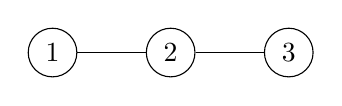
\begin{tikzpicture}[node distance={15mm}, main/.style = {draw, circle}] 
		\node[main] (1) {$1$};
		\node[main] (2) [right of=1] {$2$}; 
		\node[main] (3) [right of=2] {$3$};
		\draw (1) -- (2);
		\draw (2) -- (3);
	\end{tikzpicture}
	
	Es gilt: $|E|=2\ge \frac{(3-1)(3-2)}{2}+1$

	Im allgemeinen kann man einen kompletten Graphen auf $n-1$ Knoten, $K_{n-1}$, mit einem zusätzlichen
	Knoten über eine Kante verbinden ($\frac{(n-1)(n-2)}{2}$ ist die Anzahl der Kanten in $K_{n-1}$).
		
	\section*{4}
	\textbf{Beweise, dass jeder Graph $G = (V, E)$ mit der Eigenschaft, dass $\deg(u) + \deg(v) \ge n$ für $u, v \in V$ nicht adjazent, einen Hamiltonkreis enthält.}
	
	Das ist eine abgeänderte Version von Satz von Dirac.
	Wir können also den Beweis vom Satz von Dirac leicht abändern, um die Aussage zu zeigen.  
	Dazu betrachten wir die 2 kritische Stellen, die die Eigenschaft $\deg(v) \ge \frac{n}{2}$ nutzen, und ersetzen sie durch unsere Eigenschaft:
	
	Kritische Stelle 1:
	Wir müssen zeigen, dass $G$ zusammenhängend ist. Dazu verwenden wir das gleiche Argument wie in Aufgabe 2:  $u$ und $v$ haben nur $n-2$ Möglichkeiten für einen Nachbar, aber ihre Grade ergeben zusammen mind. $n$, also müssen sie einen gemeinsamen Nachbar haben.
	
	Kritische Stelle 2:
	Wir müssen zeigen, dass der längste Pfad $<v_1, v_2, \dots, v_k>$ zu einem Kreis verlängert werden kann.
	Dafür reicht es zu zeigen, dass es solch ein $i$ ($2 \le i \le n$) gibt, s.d. $v_1$ ein Nachbar von $v_i$ ist und $v_k$ ein Nachbar von $v_{i-1}$. Dann wäre nämlich $<v_1, v_i, v_{i+1}, \dots, v_k, v_{i-1}, v_{i-2}, \dots, v_2>$ ein Kreis, der immernoch durch alle $v_1, v_2, \dots, v_k$ durchgeht.
	
	Wir überlegen uns dazu, wie viele Nachbarn $v_k$ höchstens haben könnte, wenn es kein solches $i$ gäbe.
	Es gibt insgesamt $k-1$ Möglichkeiten, weil alle Nachbarn von $v_k$ auf dem Pfad liegen müssen. 
	Ansonsten könnten wir ja die Nachbarn zum Pfad hinten dran hinzufügen und somit bekommen wir einen längeren Pfad, Widerspruch.
	Wenn es kein solches $i$ gibt, dann kann auch kein Knote, der unmittelbar vor einem Nachbar von $v_1$ auf dem Pfad liegt, ein Nachbar von $v_k$ sein.
	Dies gilt, weil auch alle Nachbarn von $v_1$ auf dem Pfad liegen.
	Somit erhalten wir $\deg(v_k) \le k-1-\deg(v_1)$ und somit auch
	
	\[\deg(v_k)+ \deg(v_1) \le k-1 \color{red}< n\]
	
	Widerspruch. Somit gibt es in $G$ einen Hamiltonkreis.
	
	\section*{5}
	\textbf{Jeder Graph $G=(V,E)$ mit $|V| \ge 3$ und $|E| \ge \frac{(n-1)(n-2)}{2}+2$ enthält einen Hamiltonkreis.}
	
	Wir zeigen erst, dass für alle $u,v \in V$ nicht adjazent gilt: $\deg(u)+\deg(v) \ge n$
	
	Wenn das  nicht gelten würde, hätten wir zwei Knoten $u,v$ mit $\deg(u)+\deg(v) < n$.
	Dann können die restlichen $n-2$ Knoten höchstens $\frac{(n-2)(n-3)}{2}$ Kanten untereinander haben (vollständiger Graph auf $n-2$ Knoten).
	Dazu müssen sie noch $\deg(u)+\deg(v)$ viele Kanten zu $u$ und $v$ haben, da $u$ und $v$ nicht adjazent sind.
	Jetzt analysieren wir, wie viele Kanten es dann höchstens geben kann (mit Hilfe von Handshake Lemma):
	\begin{align*}
		|E| = \frac{\sum_{v \in V} \deg(v)}{2} 
			&\le \frac{2(\deg(u)+\deg(v)) +(n-2)(n-3)}{2} \color{red} < \color{black} \frac{2n +	(n^2-5n+6)}{2}
		\\ 	&= \frac{n^2-3n+6}{2} = \frac{n^2-3n+2}{2} + 2 = \frac{(n-1)(n-2)}{2} + 2 = |E|
	\end{align*}
	was ein Widerspruch wäre.
	Wir schliessen den Beweis ab, indem wir die Aufgabe 4 anwenden.
\end{document}